%% Use \documentclass[print]{dissertation} to export the document
\documentclass[]{tesefop}



%%%%%%%%%%%%%%% Configuração: dados pessoais %%%%%%%%%%%%%%

% Descomente a linha abaixo em caso de Mestrado. Para Doutorado manter a linha desativada
%\def\mestrado{}

% Substituir 'Nome completo do aluno' pelo seu nome.
\newcommand{\autor}{Nome completo do aluno}
% Se for do sexo feminino, descomente a linha a seguir.
%\def\femaleAuthor{}

% Substituir 'Título da defesa' pelo título da defesa.
\newcommand{\titulo}{Título da defesa}

% Substituir 'Título do Doutorado".
\newcommand{\titulodoc}{Clínica Odontologica}

% Substituir 'Area do doutorado'
\newcommand{\areadoc}{Prótese Dental}


% Substituir 'Nome completo do orientador' pelo nome completo do seu
% orientador.
\newcommand{\orientador}{Nome completo do orientador}
% Se for orientado por uma mulher, descomente a linha a seguir.
% \def\femaleOrientador{}

% Substituir 'Nome completo do coorientador' pelo nome completo do seu
% coorientador. Caso não tenha coorientador, comente a linha a seguir.
\newcommand{\coorientador}{Nome completo do coorientador}
% Se for coorientado por uma mulher, descomente a linha a seguir.
% \def\femaleCoorientador{}

% FIXME Substituir 'Ano' pelo ano em que ocorreu sua defesa.
\newcommand{\ano}{2017}

  % Dados pessoais e da tese



\begin{document}
	
	%elementos pré-textuais. Não há necessidade de modificar este arquivo.
	\thispagestyle{plain}
\noindent% just to prevent indentation narrowing the line width for this line
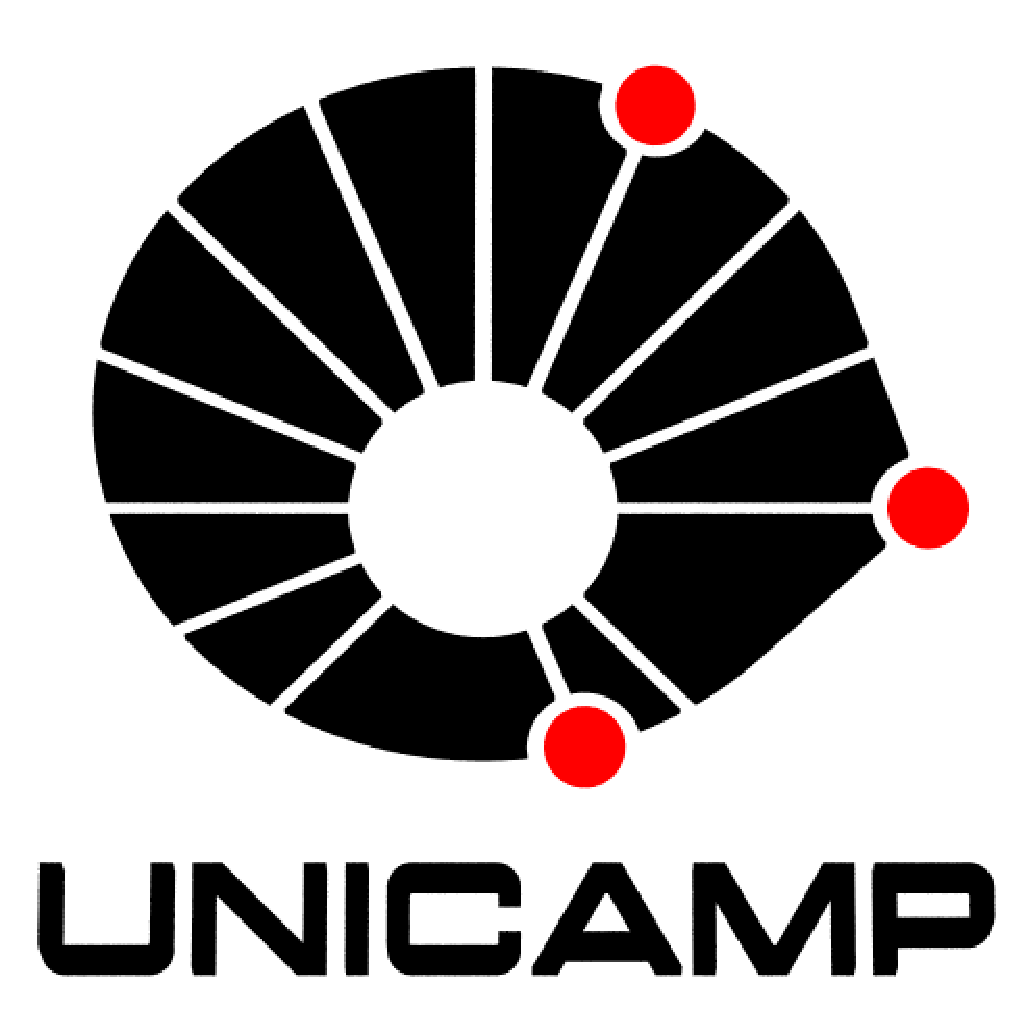
\includegraphics[width=0.10\textwidth]{imagens/logo-unicamp}%
\begin{minipage}[b]{0.7\textwidth}
	\centering
	\textbf{Universidade Estadual de Campinas} \\
\vspace{0.5cm}

\textbf{Faculdade de Odontologia de Piracicaba}
\end{minipage}%

\includegraphics[width=0.10\textwidth]{imagens/logo-fop}

\vspace{4cm}
\begin{center}
	% O tamanho da fonte deve ser 16pt.
	% Deve-se utilizar caixa alta.
	{\Large\textsc{\autor}}
\end{center}
\vspace{4cm}
\begin{center}
	% O tamanho da fonte deve ser 16pt em negrito.
	% Deve-se utilizar caixa alta.
	{\Large\textbf{\textsc{\titulo}}}
\end{center}
\vfill
\begin{center}
	% O tamanho da fonte deve ser 12pt em negrito.
	% Deve-se utilizar caixa alta.
	\textbf{Piracicaba \\ \ano}
\end{center}





\cleardoublepage
% Folha de rosto


\thispagestyle{plain}


\begin{center}
	
	{\large\textbf{\textsc{\autor}}}
	
	
\end{center}
\vfill


\vfill
\begin{center}
	{\Large\textbf{\textsc{\titulo}}}
\end{center}
\vfill

\begin{flushright}
	\begin{minipage}[c]{.5\textwidth}
		Tese apresentada à Faculdade de Odontologia de Piracicaba da Universidade Estadual de Campinas como parte dos requisitos para obtenção do título de 
		\ifx\femaleAuthor\undefined
		Doutor
		\else
		Doutora
		\fi
		em \titulodoc{} na área de \areadoc .
		
		\end{minipage}
\end{flushright}
\vspace{.5cm}

\noindent
\textbf{Orientador\ifx\femaleOrientador\undefined
	\else
	a\fi: \orientador
}
\vspace{.25cm}

\ifx\coorientador\undefined
\else
\noindent
\textbf{Coorientador\ifx\femaleCoorientador\undefined
	\else
	a\fi: \coorientador
}
\vspace{.5cm}
\fi

\noindent
\begin{minipage}[c]{.5\textwidth}
	{\footnotesize\textsc{Este exemplar corresponde à versão final da
			\ifx\mestrado\undefined
			tese
			\else
			dissertação
			\fi
			defendida
			\ifx\femaleAuthor\undefined
			pelo aluno
			\else
			pela aluna
			\fi
			\autor,
			e orientada pel\ifx\femaleOrientador\undefined
			o\else
			a\fi{} Prof\ifx\femaleOrientador\undefined
			\else
			a\fi. Dr\ifx\femaleOrientador\undefined
			\else
			a\fi. \orientador.
		}}
	\end{minipage}
	\vspace{1cm}
	
	\noindent
	
	\vspace{.5cm}
	
	
	\vfill
	\begin{center}
		{\small\textbf{\textsc{ Piracicava \\ \ano}}}
	\end{center}


\clearpage


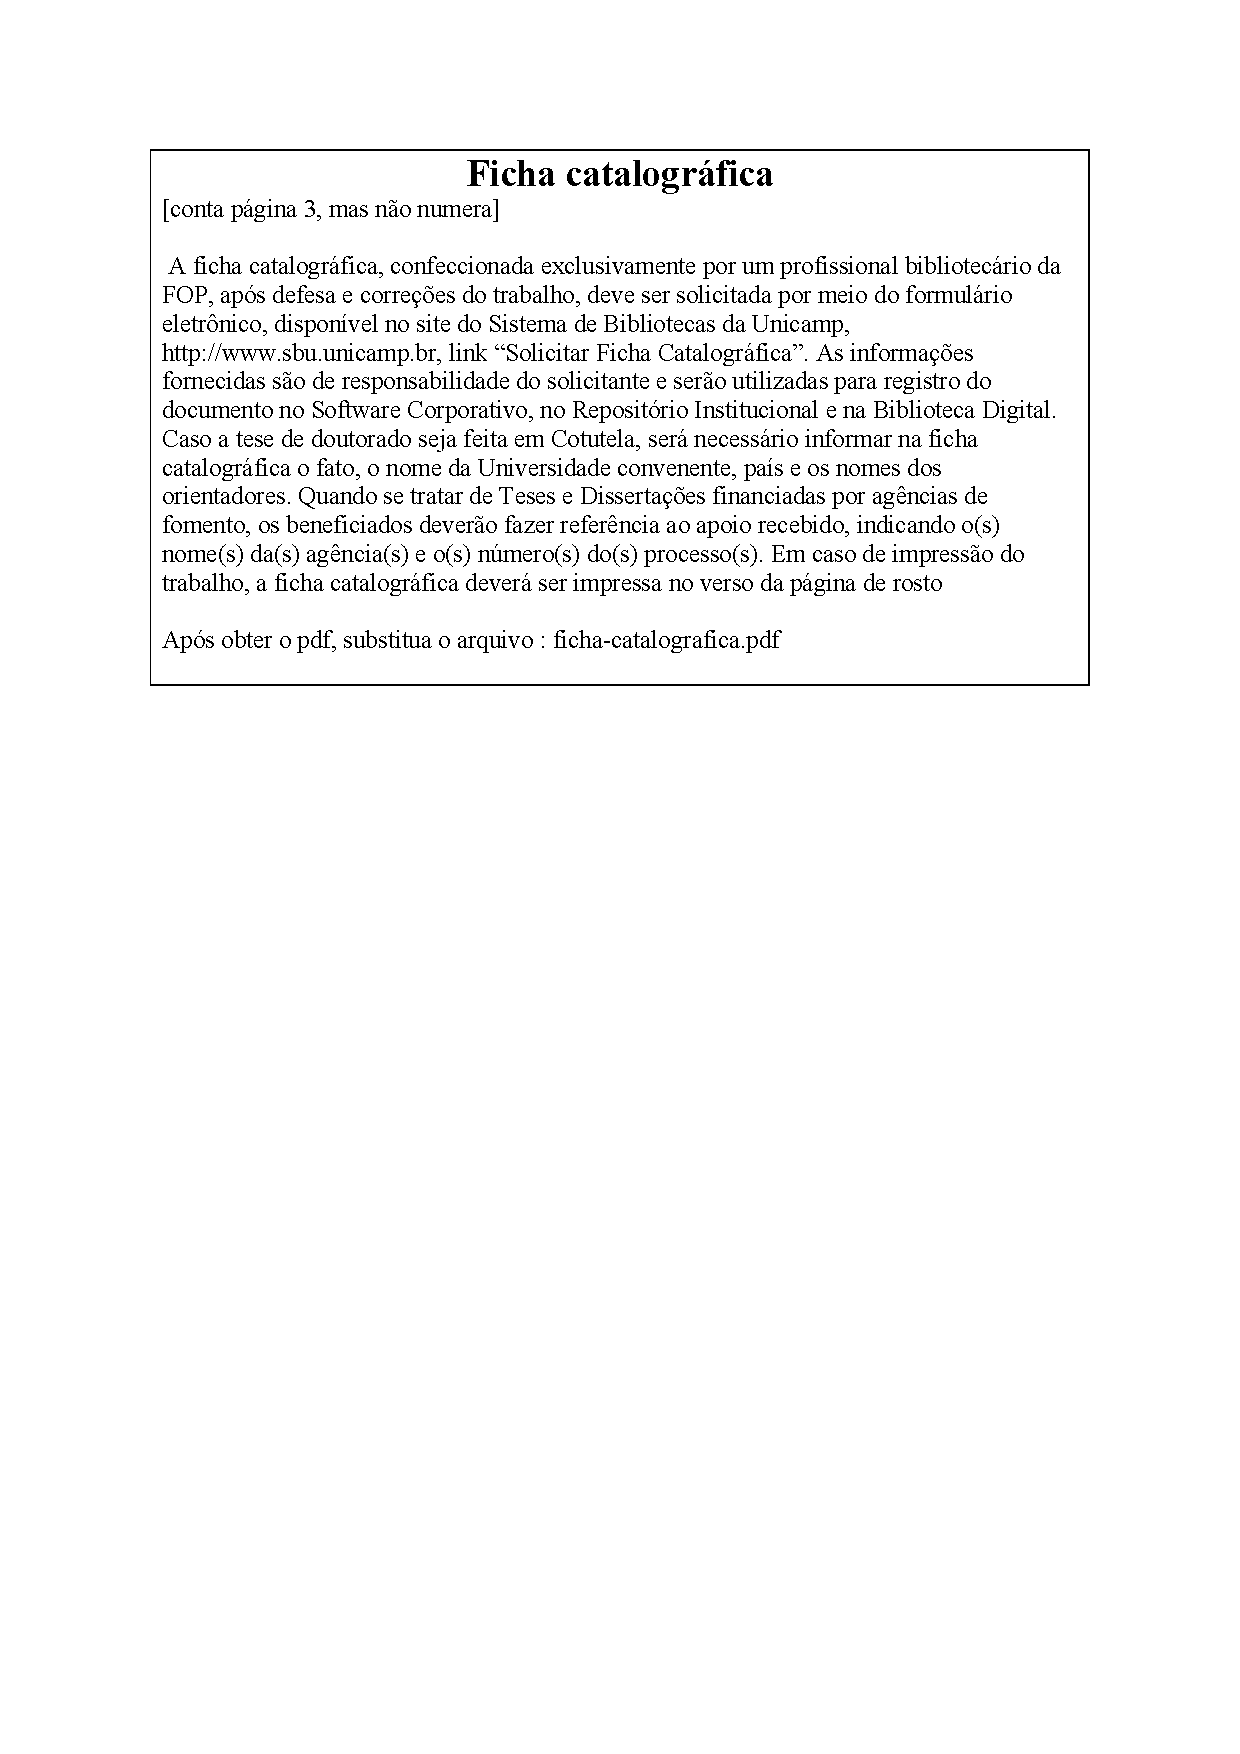
\includepdf{ficha-catalografica}

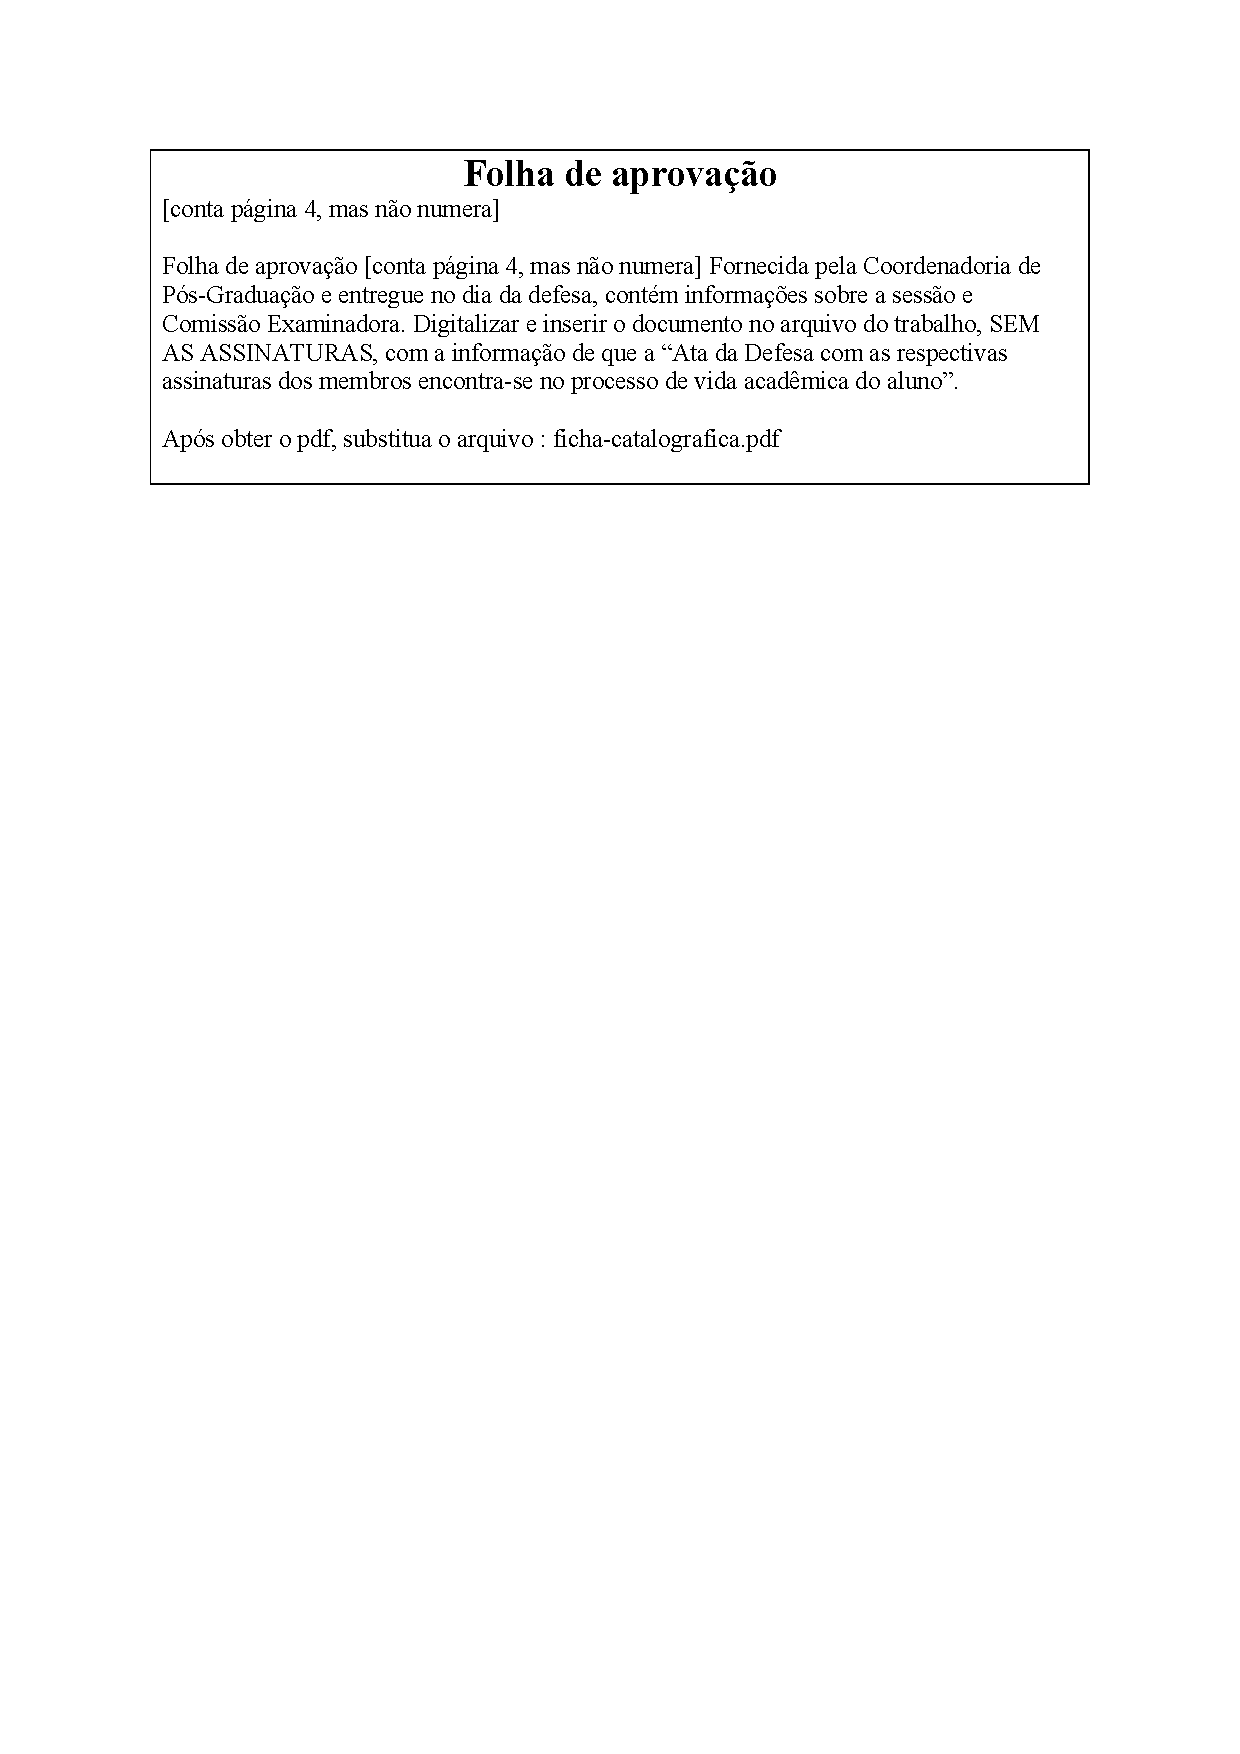
\includepdf{folha-de-aprovacao}

	
	
	\section{Dedicatoria}



\blindtext %apague completamente esta linha.
 % Opcional. Remova esta linha caso não queira incluir
	\section{Agradecimentos}

\blindtext %apague completamente esta linha. % Opcional. Remova esta linha caso não queira incluir
		
	\section{Resumo}
	\section{Abstract}

\Blindtext %apague completamente esta linha.
	%\section{Outro abstract} % Remova esta linha caso não inclua o resumo extra 
	\section{Lista de Ilustrações}

\blinditemize
 % Opcional. Remova esta linha caso não queira incluir
	\section{Lista de Tabelas}

\blinditemize % Opcional. Remova esta linha caso não queira incluir
	\section{Lista de Abreviaturas e Siglas}

\blinditemize % Opcional. Remova esta linha caso não queira incluir
	\section{Lista de Símbolos}

\blinditemize % Opcional. Remova esta linha caso não queira incluir
	
	\section{Sumario}

	\include{introducao}
	
	%%%%%%%%%%% Formato Tradicional %%%%%%%%%%%%%%%%
	% Instruções: Caso opte pelo formato tradicional, remova o % no inicio de cada linha a seguir
	%\include{revisao-literatura}		% Formato tradicional, remova % no inicio desta linha.
	%\include{proposicao}				% Formato tradicional, remova % no inicio desta linha.
	%\include{materiais-metodos}		% Formato tradicional, remova % no inicio desta linha.
	%\include{resultados}				 % Formato tradicional, remova % no inicio desta linha.
	
	%%%%%%%%%%% Formato Alternativo  %%%%%%%%%%%%%%%%
	
	% Instruções: Caso opte pelo formato alternativo, remova o % no inicio de cada linha a seguir
	%\include{artigos/artigo1}		% Formato alternativo, remova % no inicio desta linha.
	%\include{artigos/artigo2}		% Formato alternativo, remova % no inicio desta linha.
	%\include{artigos/artigo3}		% Formato alternativo, remova % no inicio desta linha.	
	
	\include{discussao}
	\include{conclusao}
	\include{referencias}
	\include{apendice1}
	\include{anexo1}
	
\end{document}